\documentclass[article,oneside]{memoir}

\usepackage{graphicx}
\usepackage{booktabs}
\usepackage{amsmath}
\usepackage[colorlinks=true, linkcolor=blue]{hyperref}
\usepackage{memhfixc}
\usepackage{listings}

\oddsidemargin 0.0in
\textwidth 6.5in 
\topmargin 0.0in 
\textheight 8.5in 

\newcommand{\obs}{\textsc{oboe}}
\newcommand{\owl}{\textsf{OWL}}
\newcommand{\seek}{\href{http://seek.ecoinformatics.org/}{SEEK}}
\lstset{language=XML, basicstyle=\tiny\ttfamily}

\title{The \obs{} Tutorial}
\author{Joshua S. Madin, Shawn Bowers, Mark P. Schildhauer, and Matt Jones}

\begin{document}

\maketitle

\tableofcontents

%%%
\pagebreak
\chapter{Introduction}
The \textbf{E}xtensible \textbf{OB}servation \textbf{O}ntology
(reversed to give \obs{}) was developed to describe scientific
observations and measurements with particular emphasis on capturing
observational context.  This emphasis is important because automated
reasoning tasks, such as searching for data or merging data sets,
require ``knowledge'' of contextual structure in order to determine if
data from different sources are compatible (e.g., equivalent or
subsumable).  For example, if a human or machine process can determine
that two data points have the same temporal and spatial context, then
the points are potentially comparable, and might be merged to increase
the power of a scientific analysis. This tutorial will focus on the
use of \obs{} for annotating ecological and environmental data sets.
A more detailed description of the of \obs{}'s ontological structure
can be found elsewhere (Madin \textit{et al.}, 2007).

\section{Observation and Measurement}

Observations and Measurements form the core of \obs{}; represented as
black ellipses in Figure~\ref{fig:oboe}.  An Observation is defined as
an assertion that a \textit{thing} (physical, abstract, or conceptual)
was observed to belong to a specified class of Entity in a specified
ontology.  For example, a field researcher might assert that an entity
they observed belongs in the class Tree in the ontology portrayed in
Figure~\ref{fig:entity} (i.e., the observed thing is an
\textit{instance} of class Tree which is a subclass of Entity).

\begin{figure}[hbtp]
  \fbox{
  \begin{minipage} {16 cm}
  \centering  
 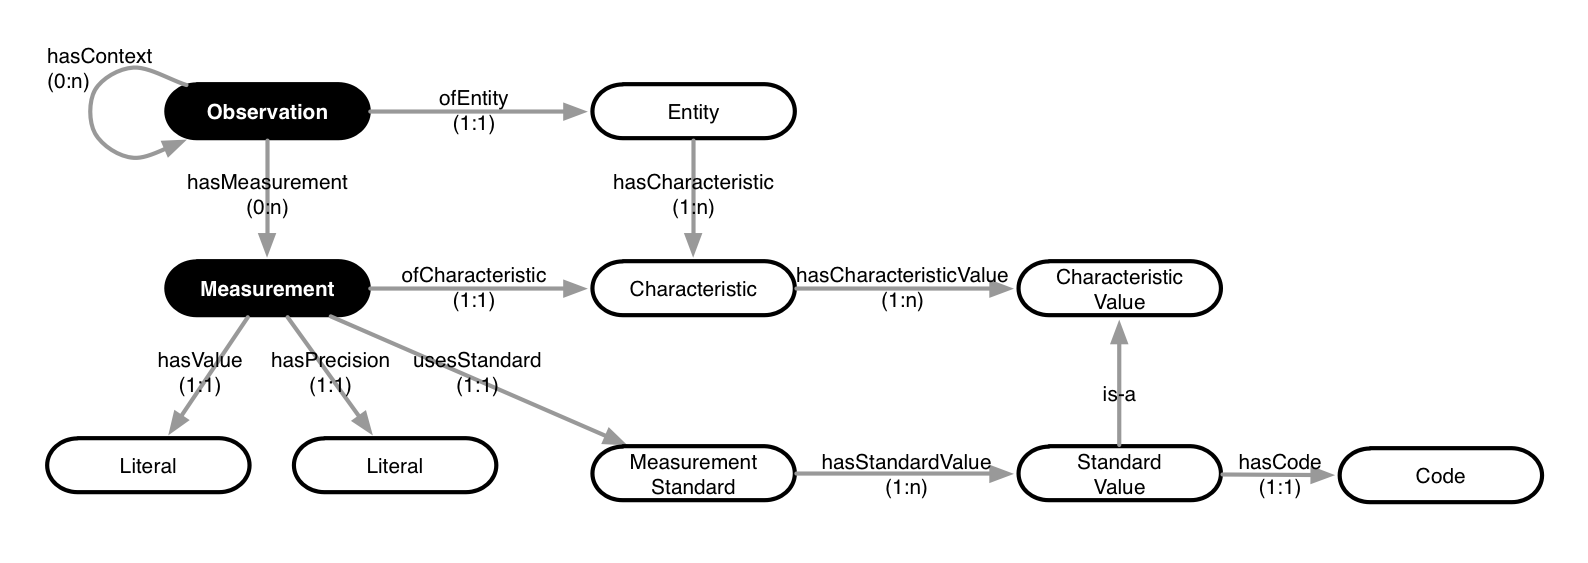
\includegraphics[width=0.9\textwidth]{./figures/tut_fig_2.png}
 \caption{A simplified representation of \obs{}'s core concepts.
   Ellipses signify ontology classes and arrows signify properties.
   Maximum and minimum cardinalities are given for each property and
   thus indicating the necessary number of connections required for a
   given data instance.}
  \label{fig:oboe}
  \end{minipage}
  }
\end{figure}

\begin{figure}[hbtp]
  \fbox{
  \begin{minipage} {16 cm}
  \centering
  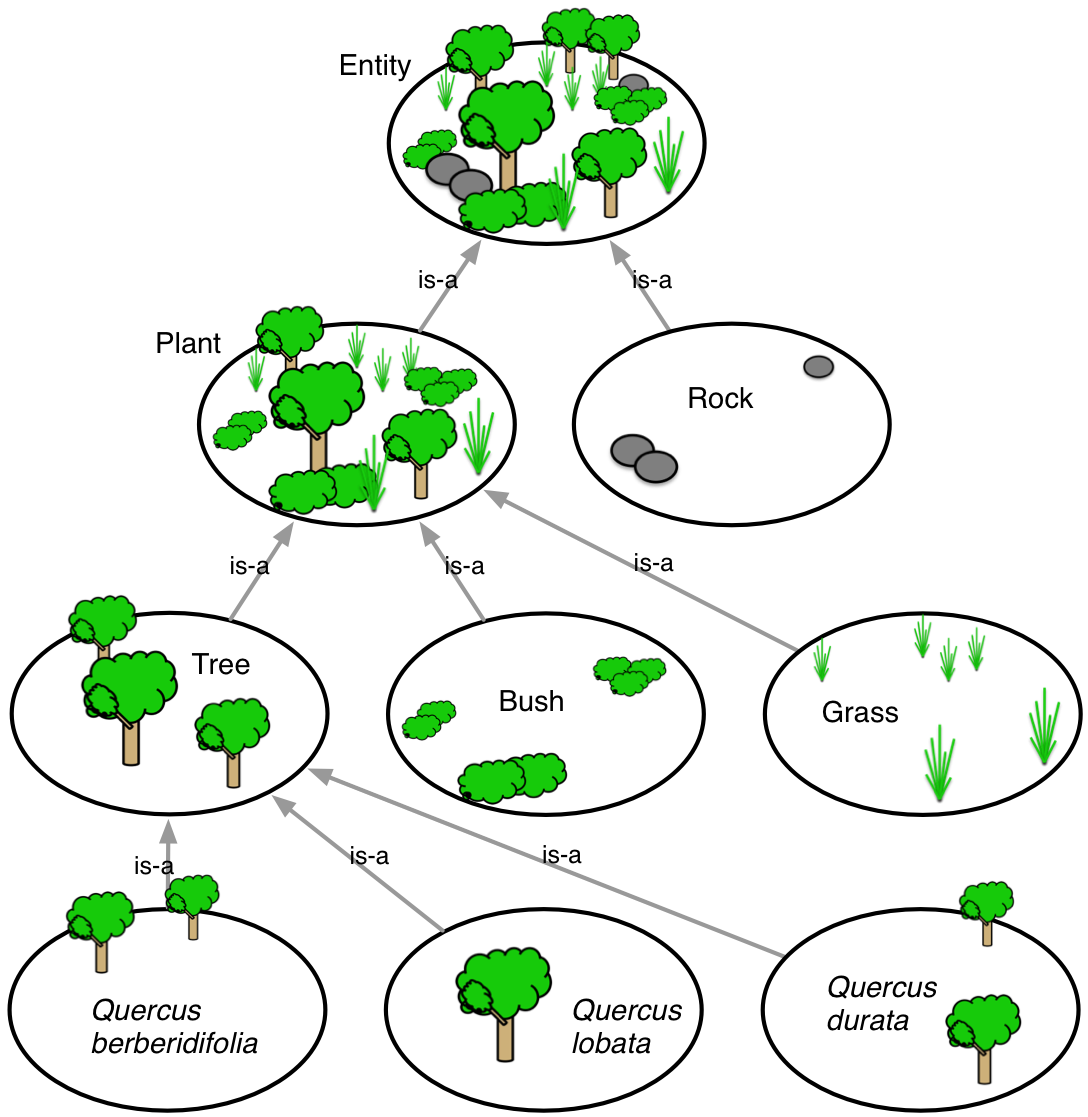
\includegraphics[width=0.45\textwidth]{./figures/tut_fig_4.png}
  \caption{A simple ontology of observable entities illustrating a
    continuum from coarser to finer level classification.  The
    property "is-a" applies to class instances (not the classes
    themselves).  As an example, this ontology states that an instance
    of the class Tree is also an instance of the class Plant, but not
    an instance of the class Rock.}
  \label{fig:entity}
  \end{minipage}
  }
\end{figure}

A Measurement is the subsequent documentation of a characteristic of
the observed entity as data (or sometimes metadata).  For example, a
data set may contain a set of tree heights (Table~\ref{tab:lobata}),
where the characteristic Height was measured for a number of instances
of the class \textit{Quercus lobata}.  A Measurement is composed from
four parts (Figure~\ref{fig:oboe}).  The first two parts are the
Characteristic that was measured (e.g., weight, color, or name) and
the Measurement Standard used to make the measurement (e.g., physical
unit or classification scheme), both of which are selected from their
respective ontology extensions of \obs{}; similar to observed Entity.
The other two parts are Value (the actual datum in the data set) and
an estimate of precision, both of which are literals (i.e., not
represented in an ontology).

\begin{table}[htbp]
  \centering
  \begin{tabular}{ @{} c @{} }
    \toprule
    Height (m) \\
    \midrule
    1.2 \\
    9.5 \\
    4.8 \\
    1.5 \\
    2.1 \\
    ... \\
    \bottomrule
  \end{tabular}
  \caption{A data set containing tree heights for the oak \textit{Quercus lobata}.}
 \label{tab:lobata}
\end{table}

\begin{figure}[hbtp]
  \fbox{
  \begin{minipage} {16 cm}
  \centering
  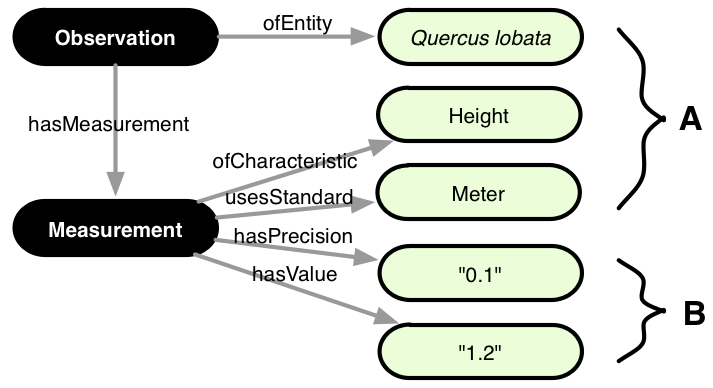
\includegraphics[width=0.4\textwidth]{./figures/tut_eg_10_tab1.png}
  \caption{The \obs{} representation of the first data point in
    Table~\ref{tab:lobata}.  A. Entities, Characteristics, and
    Standards are represented as instances of ontology classes.
    B. Measurement Precisions and Values are represented using codes
    or literals.  The other data points in Table~\ref{tab:lobata} are
    represented identically except for Value, and therefore the
    \textsf{hasValue} property is usually omitted in \obs{}
    representations.}
  \label{fig:lobata}
  \end{minipage}
  }
\end{figure}

Generally, the observed Entity is chosen to be the lowest common
denominator for the focal set of data; that is, in
Table~\ref{tab:lobata} all the height measurement data apply to
independent instances of \textit{Quercus lobata} and nothing else
(e.g., not Rock, Bush, nor \textit{Quercus durata}).  However, in
Table~\ref{tab:oaks} the observed Entity is coarser than for
Table~\ref{tab:lobata}, and the lowest common denominator is now Tree.
In this second example, the classification of instances of Tree into
``Species" is now a Measurement, and the Height of each instance is
also measured within the same instance of Tree that was observed
(Figure~\ref{fig:tut_eg_10_tab2}).

\begin{table}[htbp]
  \centering
  \caption{A data set containing heights for multiple oak species.}
  \begin{tabular}{ @{} cc @{} }
    \toprule
    Species & Height (m) \\
    \midrule
    \textit{Q. lobata} & 15.5 \\
    \textit{Q. berberidifolia} & 9.0 \\
    \textit{Q. berberidifolia} & 8.8 \\
    \textit{Q. lobata} & 16.5 \\
    \textit{Q. durata} & 5.1 \\
    ... & ... \\
    \bottomrule
  \end{tabular}
 \label{tab:oaks}
\end{table}

\begin{figure}[hbtp]
  \fbox{
  \begin{minipage} {16 cm}
  \centering
  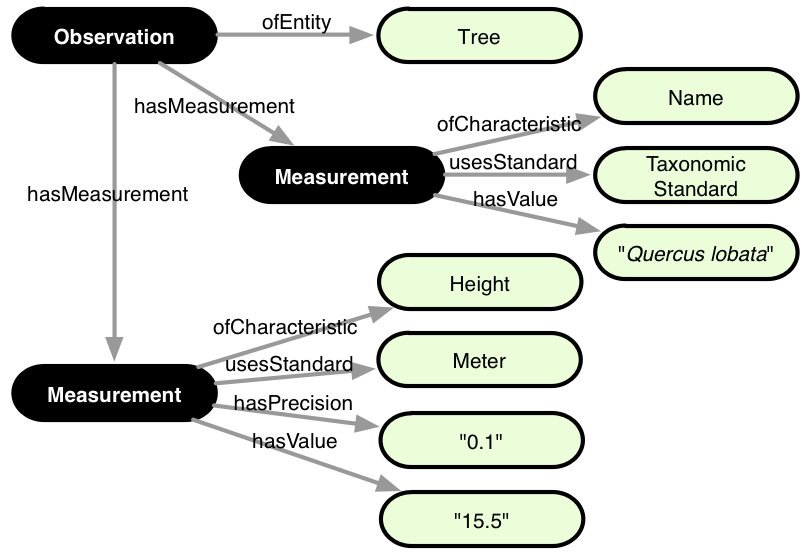
\includegraphics[width=0.45\textwidth]{./figures/tut_eg_10_tab2.png}
  \caption{The \obs{} representation of the first data point in Table~\ref{tab:oaks}.}
  \label{fig:tut_eg_10_tab2}
  \end{minipage}
  }
\end{figure}

These examples illustrate several key aspects of \obs{}:

\begin{itemize}

\item An Observation implies a \textit{definite} assertion according
  to a given ontology (or world view).  For example, the Heights
  measured in Table~\ref{tab:lobata} apply to instances of a category
  of things called \textit{Quercus lobata} according to the world view
  shown in Figure~\ref{fig:entity}.  But world views differ between
  research groups and change through time (e.g., one group might clump
  instances of the class \textit{Quercus lobata} with \textit{Quercus
    durata}).  \obs{} does not attempt to capture or track mappings
  among different world views.

\item A Measurement is, in essence, the further classification of an
  entity based its characteristics (e.g., an instance of the class
  ``7.45 Meter High Tree'') but implies an inherent degree of
  \textit{uncertainty}.  An observed entity can be measured (or
  classified) more than once (e.g., height, width, and name).
  However, each measurement must apply to the \textit{whole} entity.
  For example, it is not correct to observe a Lion and measure the
  length of its tail within the same observation.  In this case, the
  observation of Lion provides \textit{context} for a second
  observation of Tail (discussed in the next section).  Measurements
  can be made at each level of observation; e.g., the length of the
  Lion and the length of the Tail (which is associated to the
  particular instance of Lion via context).

\end{itemize}

\pagebreak
\section{Context: The Backbone of Observation}

Context forms the critical backbone of observational data.  That is,
Observations and their corresponding Measurements can only be
understood within the context they are made.  For example, there are
few interesting questions that can be asked about a set of tree
heights without any contextual information (e.g., the data in
Table~\ref{tab:lobata}).  Whereas, if there is also observational
information about location where the trees were observed, then these
data are potentially comparable with measurements taken at different
locations.  Correctly representing the contextual structure of a data
set use \obs{} takes practice, but if done correctly provides a
powerful mechanism for automatically determining the compatibility and
mergability of data.

A data set (including metadata) will typically contain information
about a object or phenomena observed, as well as the time and place it
was observed.  However, several contextual structures can potentially
describe the relationships among the three entities---e.g., Time,
Place, and Object (Figure~\ref{fig:tut_eg_11C}).  At this point, it is
important to understand that observing what we might be considered the
``same" Entity at a different time or place typically results in a
different instance of Entity.  For example, trees change through time
(i.e., they are perdurants).  In this sense, observing perdurant
Entities at different times can be treated similarly to observing them
at different places: they do not represent the same instance of
Entity.

\begin{figure}[hbtp]
  \fbox{
  \begin{minipage} {16 cm}
  \centering
  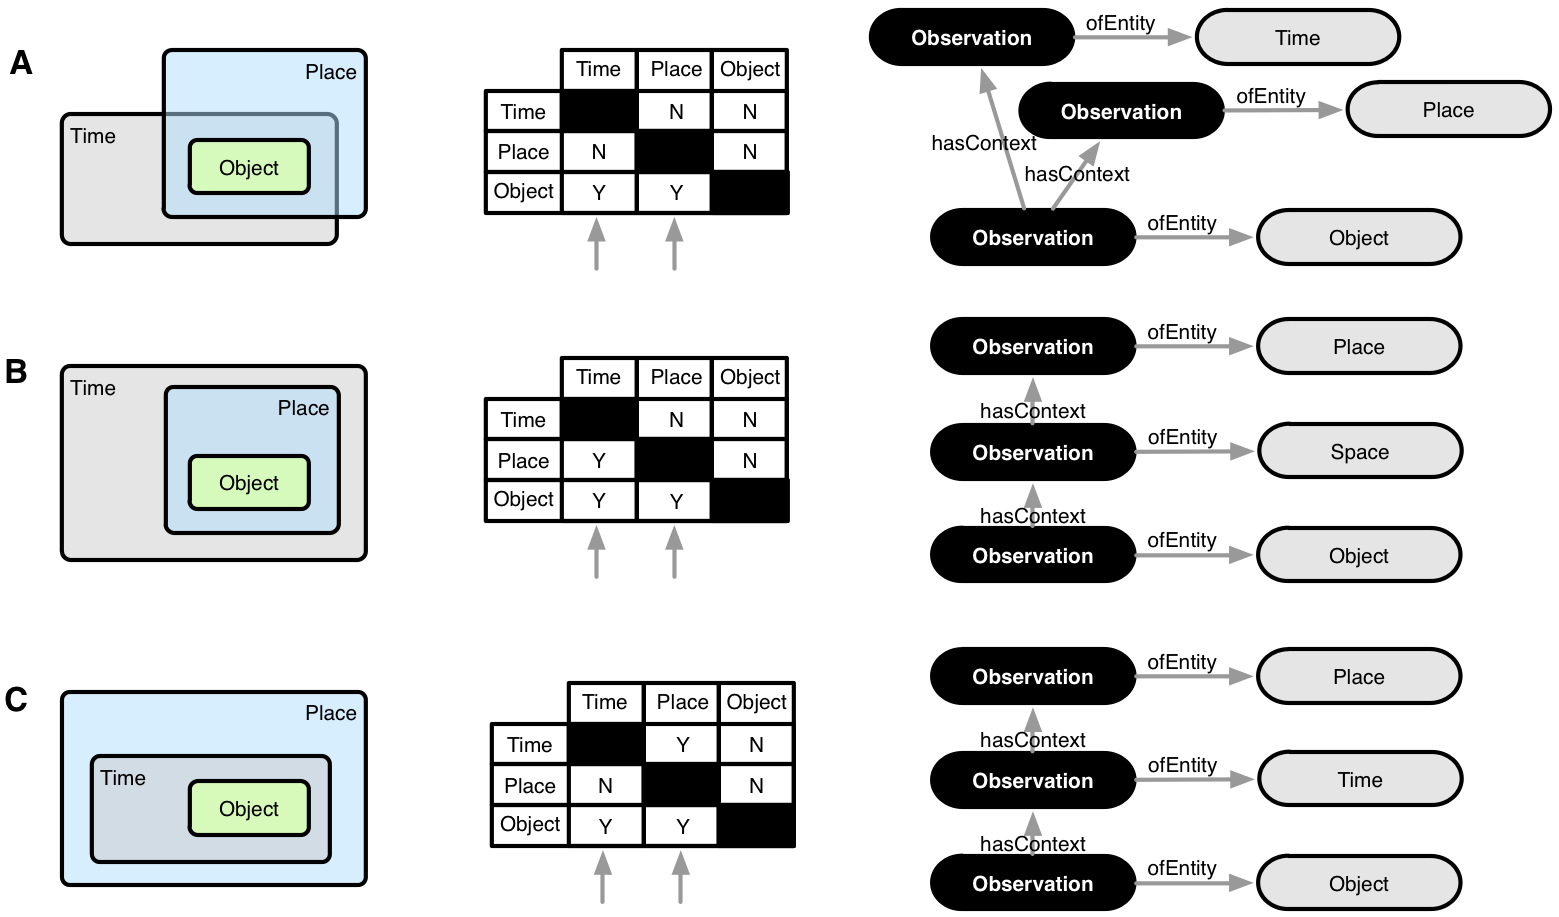
\includegraphics[width=0.8\textwidth]{./figures/tut_eg_11C.png}
  \caption{Examples of Entity instance dependence in space and time.
    Panel \textbf{A} illustrates the case when place and time provide
    independent context for Tree instance observations; that is, each
    combination of place and time contains a different (unique)
    instance of Tree.  Panel \textbf{B} shows the case when space is
    dependent of time.  This might happen if space changes through
    time, such as when space is sampled randomly at different time
    steps.  Finally, panel \textbf{C} shows the case when time is
    dependent of place.  This might happen when time-series are taken
    at different places or sampling times are selected randomly within
    a space.}
  \label{fig:tut_eg_11C}
  \end{minipage}
  }
\end{figure}

However, this is not always the case, and Space and Time are good
examples of this.  Figure~\ref{fig:tut_eg_11C} shows three possible
contextual structures for Time, Place, and Object.
Figure~\ref{fig:tut_eg_11C}A represents the contextual structure when
Time and Place provide independent context for Object.  This means
that a given instance of Place can be observed within different
instances of Time (and visa versa), however a given instance of Object
cannot be observed within different instances of Time nor Place.  The
dependency matrix for Figure~\ref{fig:tut_eg_11C}A illustrates that a
different instance of Time does not necessarily imply a different
instance of Place (denoted ``N" for No).  However, a different Time
does imply a different Object (denoted ``Y" for Yes).  Furthermore, a
different instance of Place does not imply a different instance of
Time, but it does imply a different Object.  Finally, a different
instance of Object does not necessarily imply a different Time nor
Place, because in this example it is possible to observed more than
one object at a specific Time and Place combination.  Following the
grey arrows determines the correct \obs{} context representation in
\obs{} (to the right of the matrix).  However, Time and Place are not
always independent.  Figure~\ref{fig:tut_eg_11C}B shows an example for
when Places are different (e.g., randomly chosen) at each for the
times observations were made; i.e., Place is dependent on Time.
Figure~\ref{fig:tut_eg_11C}C shows an example where Time is now
dependent on Place, which might happen when time-series are conducted
at different places.

\begin{table}[htbp]
  \centering
 \caption{A data set containing heights for multiple oak species within plots at Summer Hill on two occassions.}
 \begin{tabular}{ @{} ccccc @{} }
   \toprule
   Date & Location & Plot & Species & Height (m) \\
   \midrule
   12/04/2007 & Summer Hill & A & \textit{Q. lobata} & 2.5 \\
   12/04/2007 & Summer Hill & A & \textit{Q. lobata} & 3.1 \\
   12/04/2007 & Summer Hill & B & \textit{Q. berberidifolia} & 4.1 \\
   12/04/2007 & Summer Hill & B & \textit{Q. lobata} & 8.5 \\
   12/04/2007 & Summer Hill & C & \textit{Q. durata} & 2.2 \\
   12/06/2008 & Summer Hill & A & \textit{Q. lobata} & 7.8 \\
   12/06/2008 & Summer Hill & A & \textit{Q. lobata} & 7.7 \\
   12/06/2008 & Summer Hill & A & \textit{Q. lobata} & 2.1 \\
   12/06/2008 & Summer Hill & A & \textit{Q. lobata} & 2.6 \\
   12/06/2008 & Summer Hill & A & \textit{Q. lobata} & 3.2 \\
   12/06/2008 & Summer Hill & B & \textit{Q. berberidifolia} & 9.1 \\
   12/06/2008 & Summer Hill & B & \textit{Q. lobata} & 9.8 \\
   12/06/2008 & Summer Hill & B & \textit{Q. berberidifolia} & 2.2 \\
   12/06/2008 & Summer Hill & C & \textit{Q. durata} & 7.5 \\
   \bottomrule
 \end{tabular}
\label{tab:context}
\end{table}

Table~\ref{tab:context} contains another hypothetical data set that
was collected to monitor the growth of oak trees at a specified
location through time.  Data collection was accomplished by measuring
the names and heights of individual trees within 10 x 10 meter square
plots at two different times.  In this table, each row (or tuple) is
comprised from four Observations: one each of Temporal Point, Spatial
Location, Replicate Plot (a second spacial treatment), and Tree
(selected from the \obs{} Entity extension shown in
Figure~\ref{fig:tut_ont_1}).  Figure~\ref{fig:tut_eg_11D} illustrates
two possible ways in which the contextual structure might be
represented depending on the research protocol.  The key difference
between the two representations is whether or not the plots are (A)
permanent (i.e., the same instance of Replicate Plot can exist at
different instances of Temporal Point) or (B) randomly placed during
each census (i.e., an instance of Plot is dependent on a specific
instance of Temporal Point).

\begin{figure}[hbtp]
  \fbox{
  \begin{minipage} {16 cm}
  \centering
  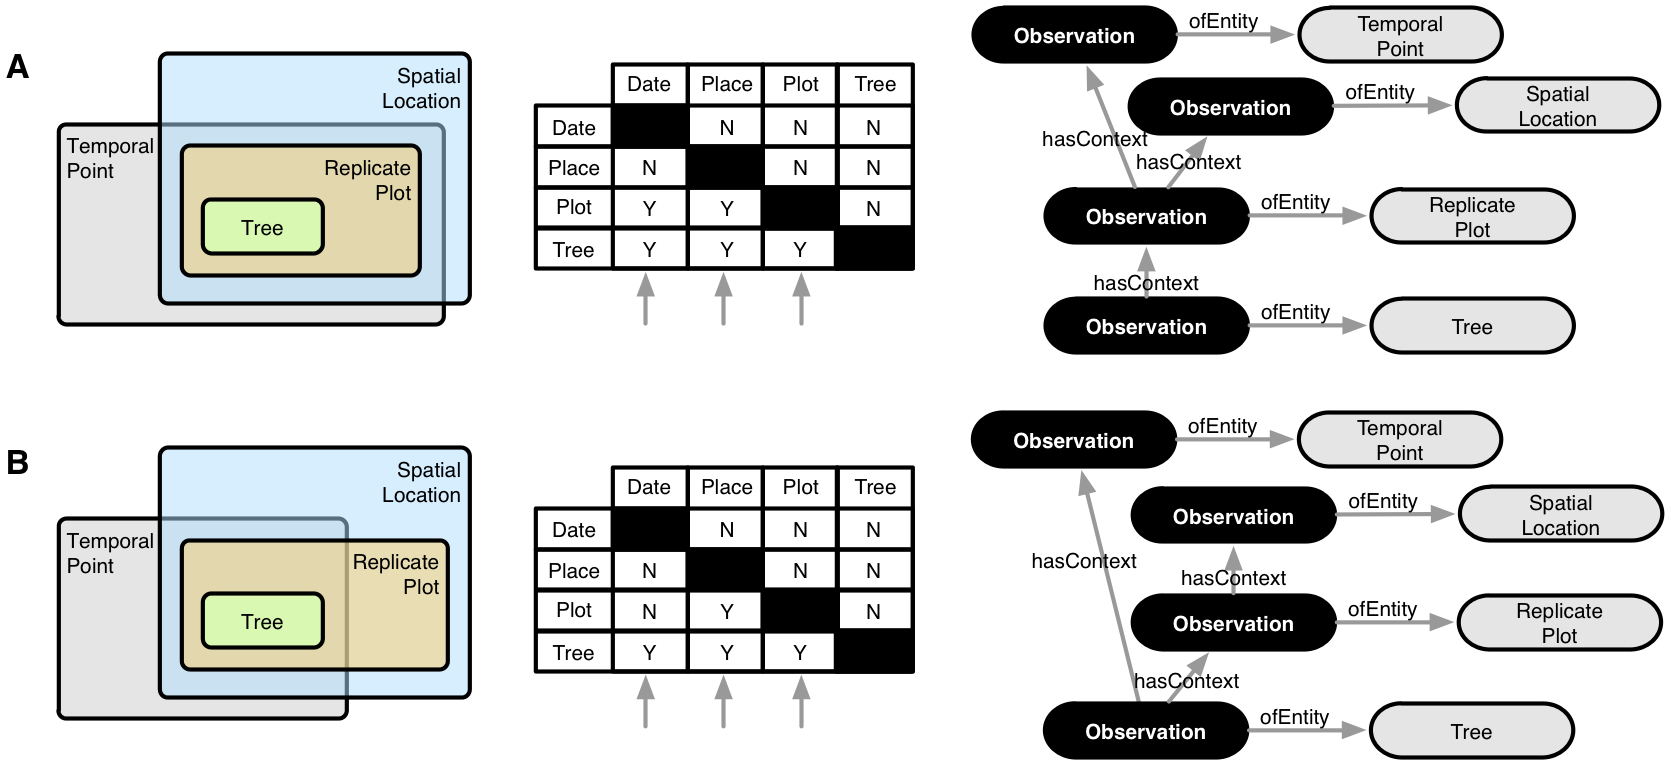
\includegraphics[width=0.85\textwidth]{./figures/tut_eg_11D.png}
  \caption{Venn diagrams illustrating two possible contextual
    structures for the Entities observed in Table~\ref{tab:context}.
    Panel \textbf{A} shows the contextual structure for when Plots are
    randomly placed at each consecutive time step; so an instance of
    Plot is dependent of an instance of Time.  Alternatively, panel
    \textbf{B} shows the structure for when Plots are permanently
    placed and thus ``endure" through time; so an instance of Plot is
    not wholly dependent on an instance of Time.}
  \label{fig:tut_eg_11D}
  \end{minipage}
  }
\end{figure}

\pagebreak

\begin{figure}[hbtp]
  \fbox{
    \begin{minipage} {16 cm}
  \centering
  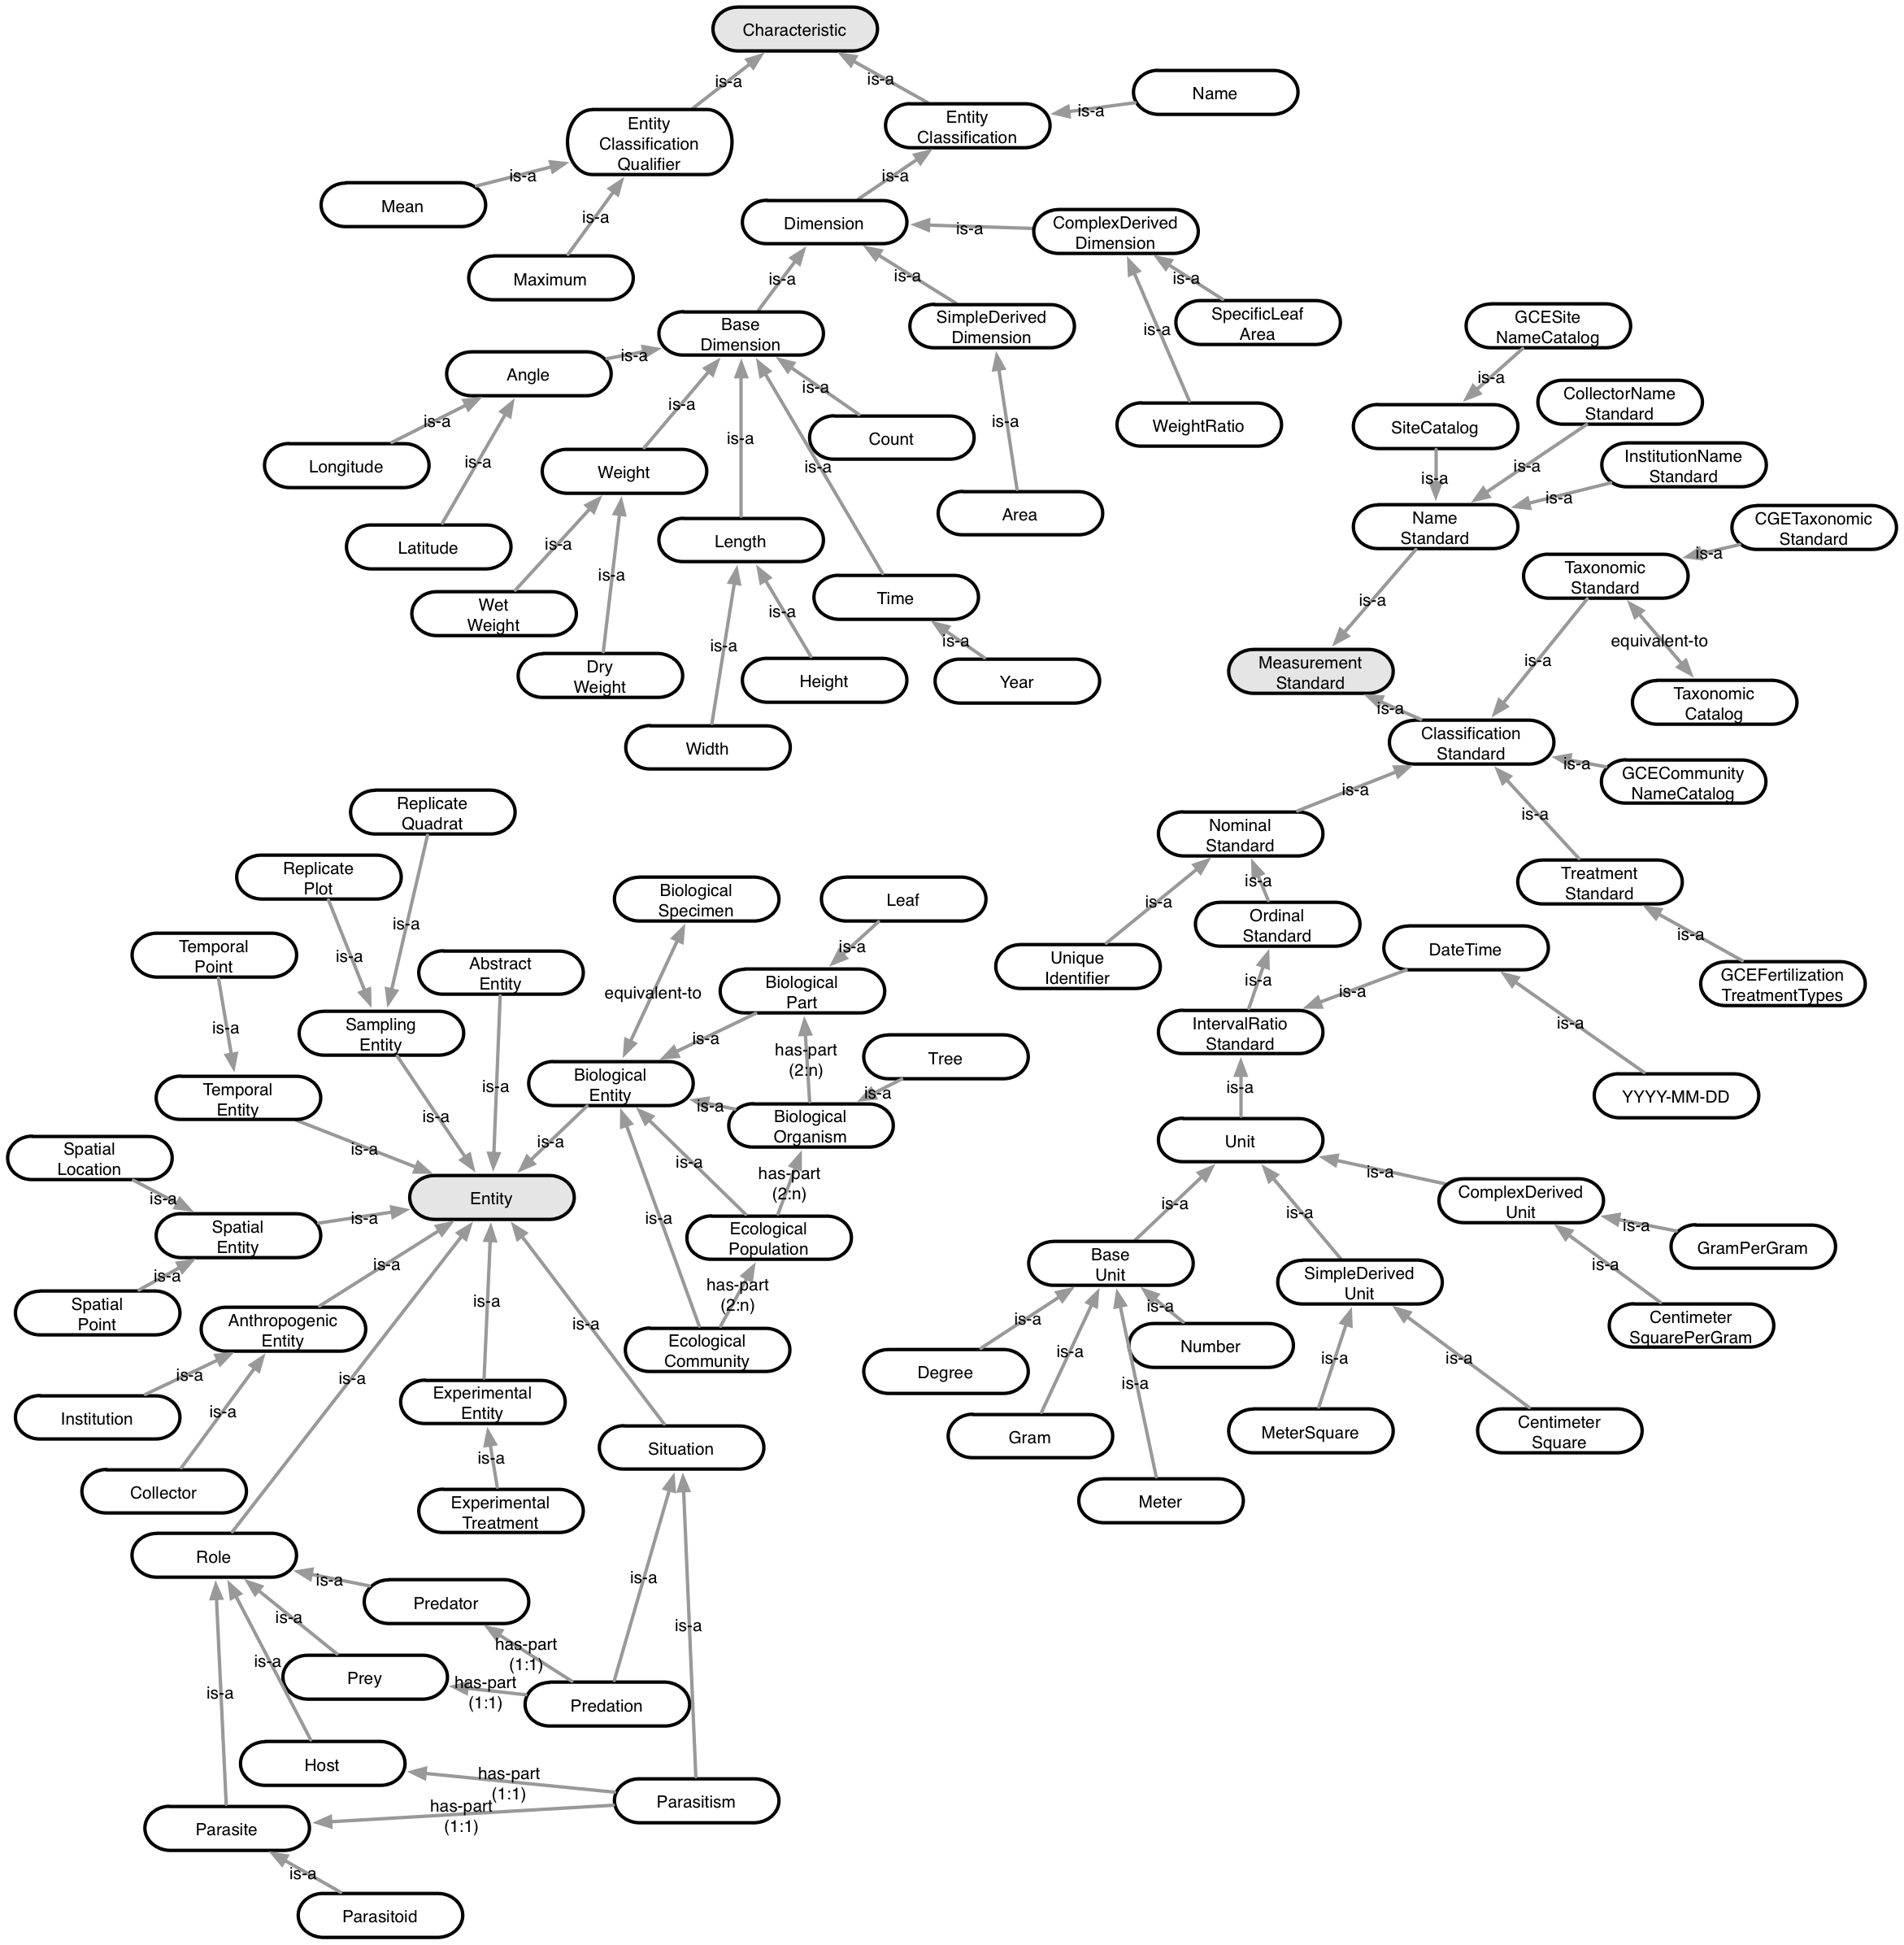
\includegraphics[width=1\textwidth]{./figures/tut_ont_1.png}
  \caption{Ontology extensions of core \obs{} classes used in this tutorial.}
  \label{fig:tut_ont_1}
  \end{minipage}
  }
\end{figure}

%%%
\pagebreak
\section{Semantic Annotation}
%%%

Semantic annotation is the mapping between data and \obs{}.  Outlined
below are the steps necessary to annotate data sets using
Table~\ref{tab:context} as the working example.  Computer software is
currently being develop to assist the annotation process.

\begin{figure}[hbtp]
  \fbox{
  \begin{minipage} {16 cm}
  \centering
  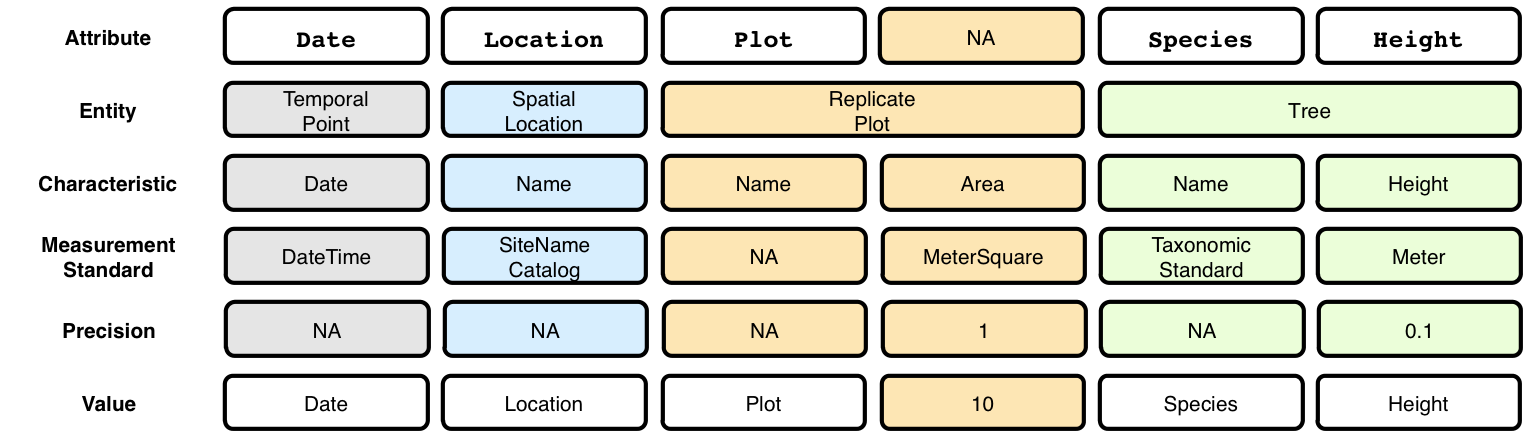
\includegraphics[width=0.75\textwidth]{./figures/tut_eg_10_att.png}
  \caption{A...}
  \label{fig: tut_eg_10_att}
  \end{minipage}
  }
\end{figure}

\begin{enumerate}

\item Identify the data attributes (in this case, columns) to be
  capture by the semantic annotation (top row in Figure~\ref{fig:
    tut_eg_10_att}).  Meta data that applies to whole-attributes
  should also be identified.  In this example, all replicate plots
  were 10 meters square, and so there was no need to include a column
  expressing this in the raw data set (and thus it was relegated to
  meta data).  However, such information is critical for determining
  important measures like areal density, especially when comparing and
  potentially merging data sets.

\item The appropriate Entities for each data attribute are then
  selected from a specified extension ontology (second row in
  Figure~\ref{fig: tut_eg_10_att}; selected from the Entity extension
  in Figure~\ref{fig:tut_ont_1}), remembering that sometimes more than
  one attribute pertains to the same Entity.  In this example, Species
  and Height both pertain to a instance of Tree.

\item Choose the Characteristics from the extension ontology that best
  describes that the attribute measured, as well as the Measurement
  Standard used to represent the Characteristic (third and fourth rows
  of Figure~\ref{fig: tut_eg_10_att}; both selected from the
  respective extensions in Figure~\ref{fig:tut_ont_1}).

\item Value points to the set of data for which the annotation
  applies.  In this case, the annotation is applied to each data point
  in the column vectors (bottom row of Figure~\ref{fig:
    tut_eg_10_att}).  Precision only applies to continuous variables,
  and is by default the number of significant decimal places (fifth
  row of Figure~\ref{fig: tut_eg_10_att}).

\item Determine the contextual structure.  In this data set, the plots
  are permanent and therefore the representation in
  Figure~\ref{fig:tut_eg_11D}B is correct.

\item Complete the \obs{} annotation graphically using the information
  in Figure~\ref{fig: tut_eg_10_att} and the context structure in
  Figure~\ref{fig:tut_eg_11D}B to give Figure~\ref{fig:
    tut_eg_10_ann}).
	
\item Represent the annotation using the Semantic Annotation Language
  (SAL) that can then be saved in the data sets metadata.  The SAL is
  described elsewhere and will be done automatically when the
  annotation software is ready.

\end{enumerate}

\begin{figure}[hbtp]
  \fbox{
  \begin{minipage} {16 cm}
  \centering
  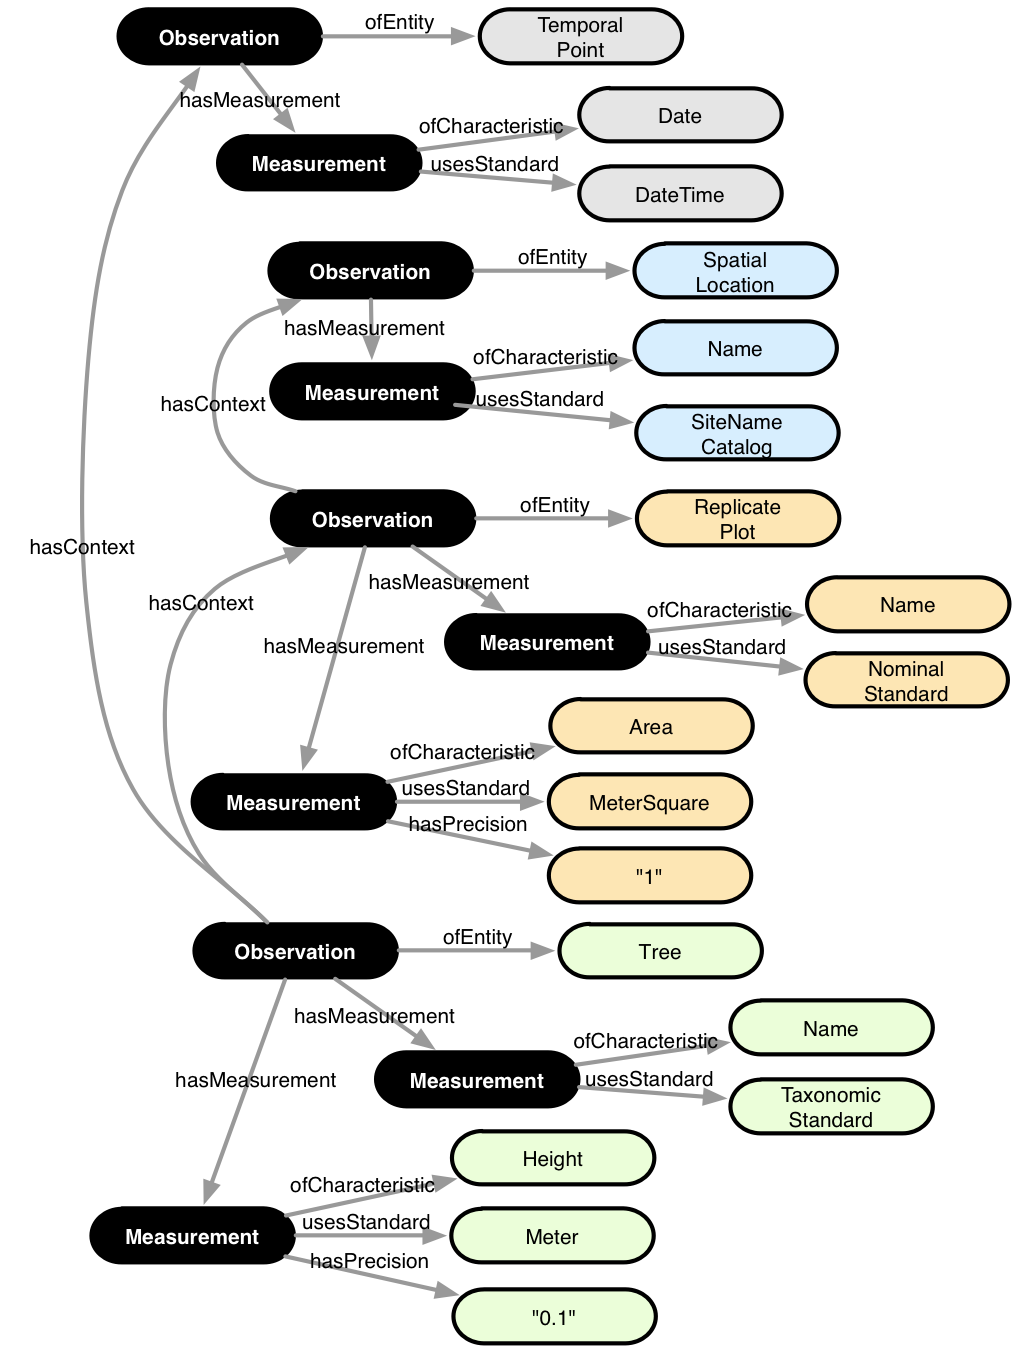
\includegraphics[width=0.55\textwidth]{./figures/tut_eg_10_ann.png}
  \caption{The \obs{} representation of the first data point in Table~\ref{tab:context}.}
  \label{fig: tut_eg_10_ann}
  \end{minipage}
  }
\end{figure}

\newpage
\textbf{ANNOTATION 1---}
\begin{lstlisting}[frame=single]
<annotation emlPackage="..." dataTable="..." xmlns:oboe="..." xmlns:ext="...">

  <observation label="o1" attributes="Date">
    <entity class="ext:TemporalPoint"/>
    <measurement>
      <characteristic class="oboe:Date"/>
      <standard class="ext:DateTime"/>
      <value attribute="Date"/>
    </measurement>
  </observation>

  <observation label="o2" attributes="Location">
    <entity class="ext:SpatialLocation"/>
    <measurement>
      <characteristic class="oboe:EntityName"/>
      <standard class="ext:SiteNameCatalog"/>
      <value attribute="Location"/>
    </measurement>
  </observation>

  <observation label="o3" attributes="Date Location ReplicatePlot">
    <entity class="ext:ReplicatePlot"/>
    <measurement>
      <characteristic class="oboe:EntityName"/>
      <standard class="oboe:NominalStandard"/>
      <value attribute="Plot"/>
    </measurement>
    <measurement precision="1">
      <characteristic class="ext:Area"/>
      <standard class="ext:MeterSquare"/>
      <value constant="10"/>
    </measurement>
    <context observation="o1" property="oboe:hasContainmentContext"/>
    <context observation="o2" property="oboe:hasContainmentContext"/>
  </observation>

  <observation label="o4" attributes="*">
    <entity class="ext:Tree"/>
    <measurement>
      <characteristic class="oboe:EntityName"/>
      <standard class="ext:TaxonomicStandard"/>
      <value attribute="Species"/>
    </measurement>
    <measurement precision="0.1">
      <characteristic class="ext:Height"/>
      <standard class="ext:Meter"/>
      <value attribute="Height"/>
    </measurement>
    <context observation="o3" property="oboe:hasContainmentContext"/>
  </observation>

</annotation>
\end{lstlisting}


\clearpage

%%%
\chapter{Examples of Semantic Annotation}

In this section, a number of real data sets are annotated using \obs{} starting with basic examples and getting progressively harder.

\section{Height Measurement}
\section{Tree Measurements I}
\section{Tree Measurements II}
\section{Leaf Traits}
\section{GCE Fertilisation Plots}
\section{Specimen Record}
\section{Summary of Organism Heights from Example 3}
\section{Predator-Prey Study}
\section{Parasitoid--Parasite--Host Study}


\end{document}